\documentclass[11pt]{article}
\usepackage[utf8]{inputenc}
\usepackage{graphicx}
\usepackage{biblatex}
\usepackage{float}
\addbibresource{bibliography.bib}
\title{Golf Ball Sameness}
\usepackage[margin=4cm]{geometry}

\author{Group D1 (R\&A):
\\James Kearney- 1876661,
\\Nisha Wiseman- 2043115,
\\Samuel Carson- 2028853,
\\Steven Leacy- 2047408,
\\Daniel Oakley- 2000475,
\\Mohammad Ruhan Ahmed- 2001322}
\date{January 2021}

\begin{document}

\maketitle

\begin{figure}[H]
    \centering
    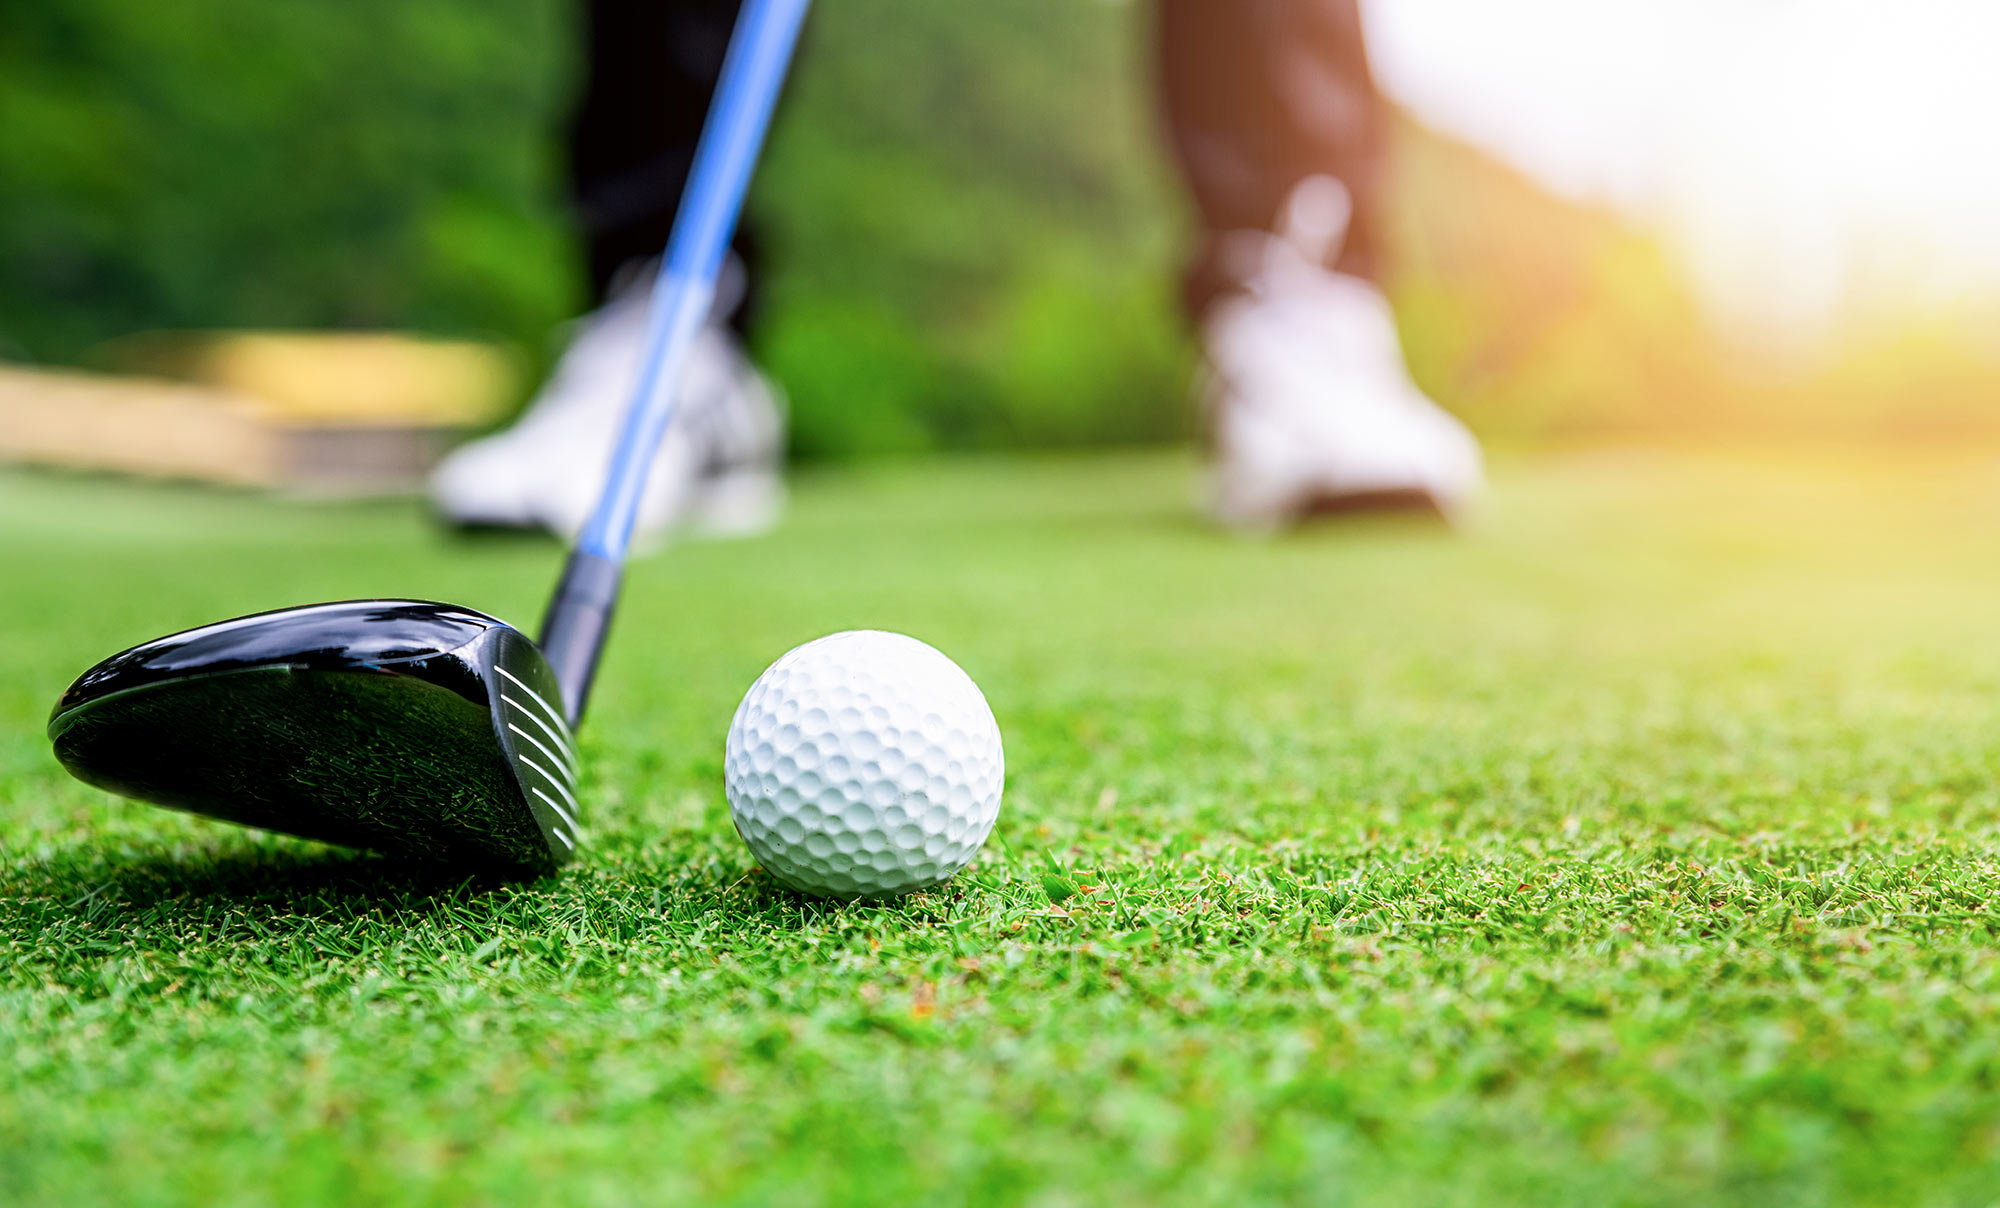
\includegraphics[width=120mm]{golf.jpg}
\end{figure}

\newpage

\section{Introduction: Interpreting 'Sameness'}

The Royal and Ancient Golf Club of St Andrews(R\&A), governs golf worldwide alongside USGA, which involves setting the Rules of Golf and Rules of Amateur Status and Equipment Standards. The brief considers the ‘One Ball’ rule which is required for elite golf events, which states you have to play with the same type and brand of golf ball you started the hole with, in order to not obtain an advantage as different balls will have different properties suited to different types of shots. In particular the brief is looking at data for the initial velocity of golf balls from a sample and testing whether these conform enough to be considered the same ball.


To consider this problem from a mathematical perspective, it is necessary that we understand what we mean when we require two golf balls to be the 'same'. Defining this condition appropriately is necessary so that it is clear what the techniques and methods being considered are aiming to show hold, or fail to hold.


The current test for the ‘One Ball’ rule being carried out by R\&A is: 
For each golf ball, the initial velocity shall be compared to the 250.0 ft/s limit plus a maximum tolerance of 2$\%$. In a sample of 24 golf balls, if four or more initial velocities exceed 255.0 ft/s, then the sample shall be ruled nonconforming to the Equipment Rules, Part 4, Section 5.\cite[~pg.4]{R_A}

This report aims to develop a more thorough and accurate test to determine whether a ball’s initial velocity conforms to the ‘One Ball’ rule through analysing and testing for: excessive ranges; extreme outliers; bimodal distributions and comparing tests from different years.
This is of importance to be able to ensure that the performance of a given type of golf ball from a manufacturer is consistent to within reasonable margins. Indeed in professional play especially, it is important to keep the performance of the balls consistent to guarantee fair play is possible.


%\begin{figure}[H]
%    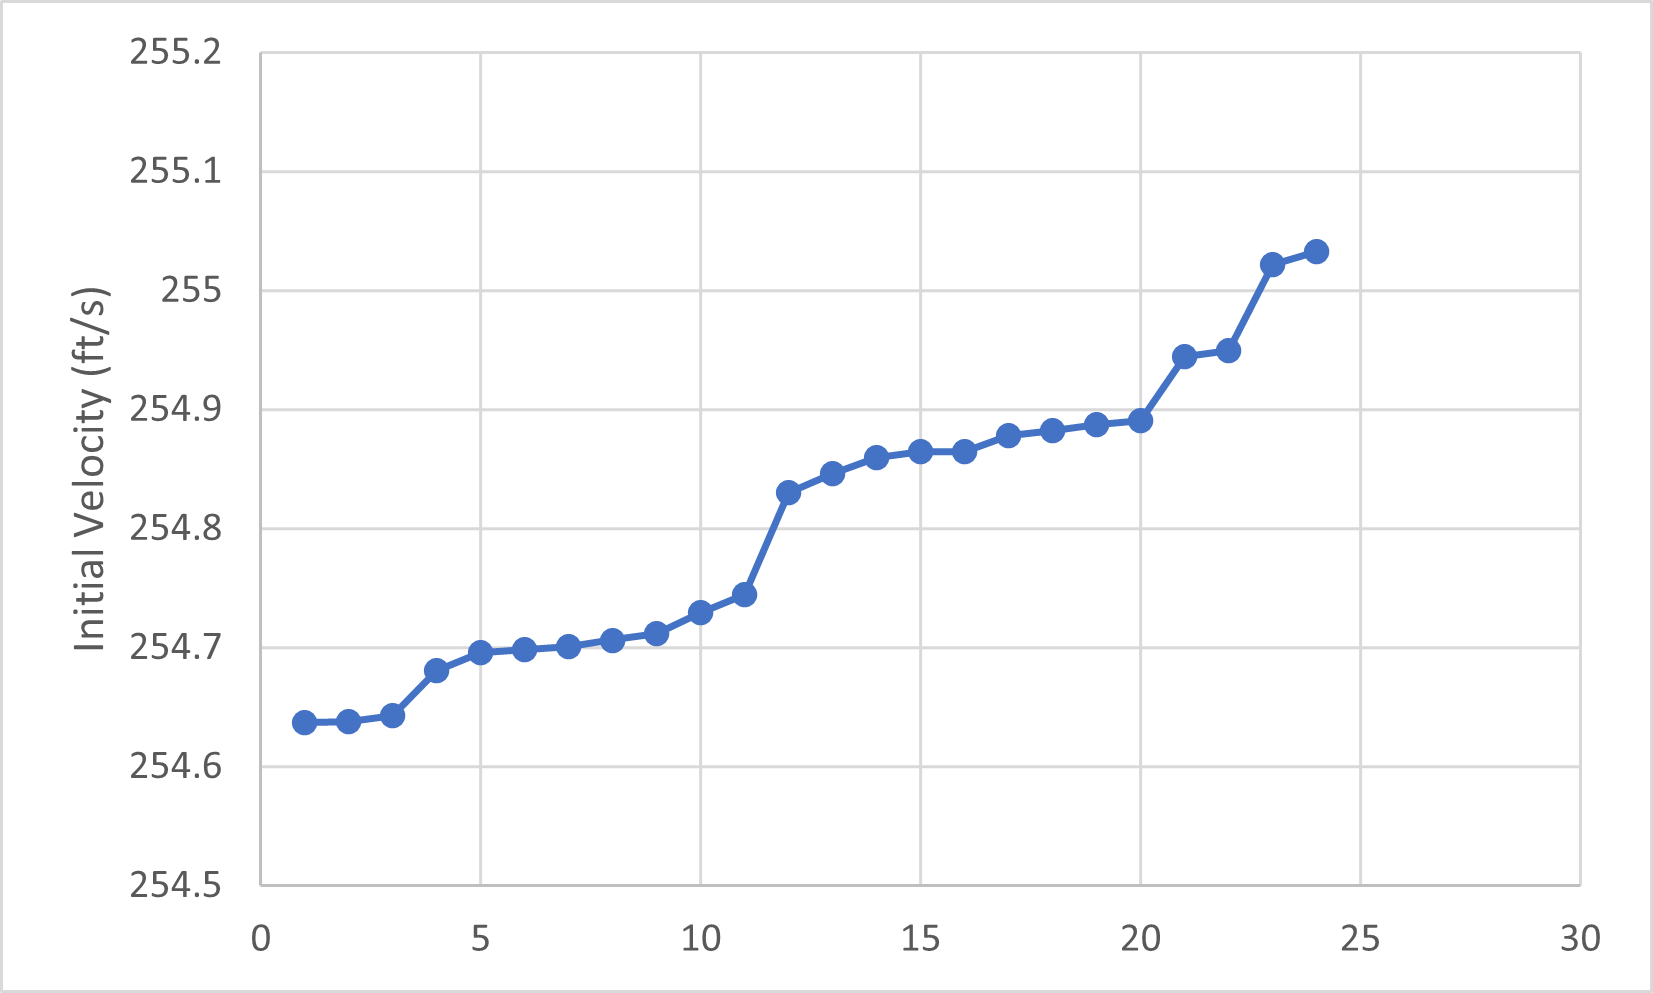
\includegraphics[width=80mm]{Sample3.png}
%    \caption{Sample 3}
%    \label{figure 1}
%\end{figure}

%Visually, from figure 1 we can see that the sample seems to consist of at least 2 distinct distributions. One for the first 11 golf balls of the sample, and another for golf balls 12 to 20, with possibly some outliers at the end. We want our method to be able to detect a bi-modal or multi-modal distribution, which would be indicative of golf balls following a different distribution. If we detect this then we will conclude that the sample does not consist of golf balls which are the same. 

\newpage

\section{Excessive Ranges}

If the range of the sample is too large, then the golf balls in the sample do not perform consistently and hence can’t be considered the same. Indeed this inconsistency may be exploited by players by using golf balls from the same sample to achieve different affects in a shot. Thus we need a method to test if the sample has an excessive range, we can’t simply test the range of the sample since one outlier can throw this off and the sample could fail the test, whilst the rest of the sample is performing consistently. For example sample 32 performs consistently but would potentially fail a range test since it has an outlier. The effects of outliers in the sample will be dealt with in a later section.


\begin{figure}[H]
    \centering
    \includegraphics[width=80mm]{Sample32.png}
    \caption{A graph showing Sample 32 which could potentially fail a range test}
    \label{figure 2}
\end{figure}


Therefore we choose to test the interquartile range, which is the difference between the 75th and 25th percentiles of the sample. We calculate the interquartile range for the first 50 data sets, then this gives us the distribution of the interquartile ranges as shown below, where the samples have been sorted in order of increasing interquartile range. 


\begin{figure}[H]
    \centering
    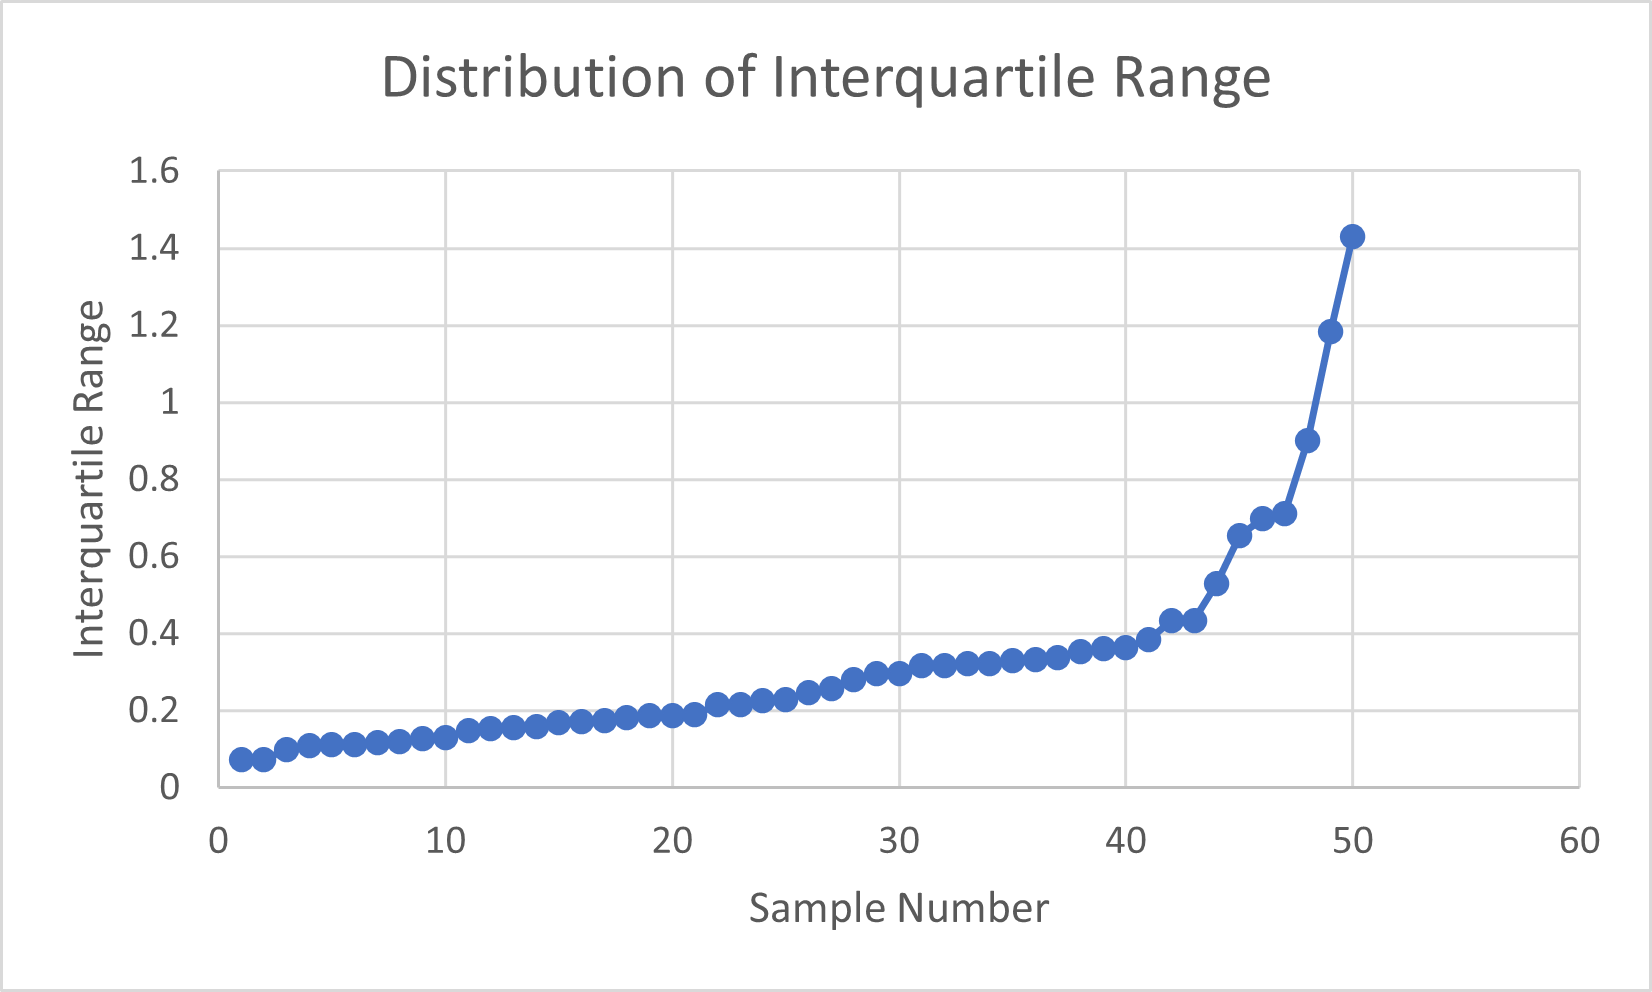
\includegraphics[width=80mm]{distributionofinterquartilerange.png}
    \caption{A graph showing the Distribution of Interquartile ranges of first 50 samples}
    \label{figure 3}
\end{figure}


We will classify an interquartile range as an outlier if the data point is greater than $\mu+3\sigma$ of the above distribution
(Where $\mu$ is the mean of the all of the interquartile ranges for the first 50 samples and $\sigma$ is the standard deviation).
So 0.15$\%$ of the data will be deemed outliers since 99.7$\%$ is within 3 standard deviations of the mean following the Empirical rule and since we are only testing if the interquartile range of the sample is too large we don’t consider lower outliers.


\begin{figure}[H]
    \centering
    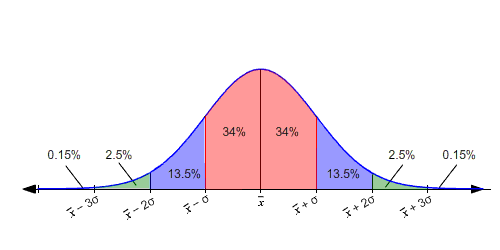
\includegraphics[width=80mm]{Outliers.png}
    \caption{A graph from varsitytutours.com \cite{Varsitytutors} showing the percentage of data within 3 standard deviations of the mean for a normal distribution}
    \label{figure 4}
\end{figure}



We find the standard deviation of the interquartile ranges of the first 50 data samples using the known formula:
$\sigma =\sqrt{\frac{\Sigma(X-\mu)^2}{N}}$
(Where N=50 the total number of samples considered) 

We thus get $\mu=0.31830$ and $\sigma=0.26963$ (both to 5 decimal points).
This now allows us to classify an excessive interquartile range using our definition of an outlier, $ \mu+3\sigma=1.12719 $.

So any sample with an interquartile range greater than this we deem as an outlier and thus having an excessive range. This gives two outliers from the first 50 data samples, samples 27 and 47 . So samples 27 and 47 have a too large range and cant be considered the same as they don’t perform consistently enough to comply with the R\&A requirements.


\section{Extreme Outliers}

%method to quantify when a sample has outliers that are too far from the mean, and so shouldn't be considered the same.

In order to ensure that the analysis of the conformity of the golf balls is as accurate as possible, we must consider outliers. An outlier is a data point that “appears to deviate markedly from other members of the sample in which it occurs”.\cite{Frank_Grubbs} There are a number of different statistical methods from which you can detect these given outliers. This analysis is important to this investigation as our aim is to find an accurate way to classify the golf balls as suitable or unsuitable to be used in golfing competitions. It is for this reason that the existence of outliers in a sample is undesirable, as each golf ball should have a reliable performance in order to suit the requirements that the R\&A set.

The method that will be implemented to find outliers in the data is called the 'Generalized ESD Many-Outlier Procedure' as outlined by Boris Iglewicz and David Hoaglin.\cite{Outliers} The Generalised ESD test, takes a chosen upper bound $r$, and carries out $r$ tests, testing for $r$ outliers. In this method, we usually choose the significant level, denoted by $\alpha$, to be 0.05, and the degree of freedom, denoted by $d_f$ will be $(n-2)$, where $n$ is the sample size.\cite{Zmuk}
Taking Sample 55, we can compute whether there are any outliers in the sample. 

\begin{figure}[H]
    \centering
    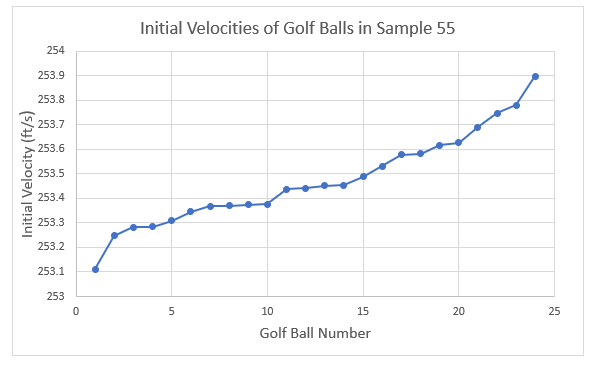
\includegraphics[width=80mm]{Sample55new.png}
    \caption{Graph showing the initial velocities of balls tested from Sample 55}
    \label{figure 5}
\end{figure}

With this sample we can implement the outlier detection method. The first step we take is to define a number of different properties of the sample. Here, we note that to find the standard deviation of the sample, we use the following formula, where each $x_i$ corresponds to each value of $x$ and $N$ is the sample size.
$$\sigma = \sqrt{\frac{\sum (x_i - \mu)^2}{N}}$$

For this test, we can identify that there is an outlier in the sample when its corresponding G-value is higher than the critical G-value. If this happens, then that outlier is omitted from the sample and the test is performed again. 
$$G_{crit}= \frac{(n-1)t_{crit}}{\sqrt{n(d_f + t_{crit}^2)}}$$
This critical value is as seen in Grubbs's test, where $t_{crit}$ is the critical value of the t-distribution $T(n-2)$ with confidence level $\alpha/n$.\cite{Zmuk} These values can be easily computed using technology or found in t-distribution tables. 
$$G=\frac{max\mid{x_i - \mu}\mid}{\sigma}$$
This G-value, is tested for each value of x, although intuitively we know that $x_i -\mu$ will be maximised at either the minimum or maximum value. With all the values defined, we can begin the Generalised ESD test, for Sample 55, it is suitable to choose $r=6$, in order to make sure no outliers are ignored.  

\begin{figure} [H]
\begin{center}
\begin{tabular}{ |l|l| } 
\hline
\multicolumn{2}{|c|}{Generalised ESD Test for Sample 55} \\
\hline
\hline
 Maximum & 253.8972776  \\ 
  \hline
 Minimum & 253.1106796  \\
  \hline
 Mean ($\mu$) & 253.4747052  \\ 
 \hline
  Standard Deviation ($\sigma$) & 0.187450056 \\
 \hline
 $x_{max} - \mu $ & 0.422572395 \\
 \hline
 $ \mu - x_{min}$ & 0.364025647 \\
 \hline
 $G$ & 2.25431992 \\
 \hline
 $t_{crit}$ & 3.487973183 \\
 \hline
 $G_{crit}$ & 2.801551162 \\
 \hline
 \end{tabular}
 \\
 \caption{Table showing values for the Generalised ESD Test for Sample 55.}
\label{tab:ESD Test of Sample 55}
 \end{center}
 \end{figure} 
 Here we can see that $G < G_{crit}$, but we do not stop carrying out the test now. We continue to do six trials, in order to ensure the effects of 'masking' are not stopping us from identifying any outliers. Masking is when more than one outlier is present, each outlier 'masking' the effect of the others, consequently effecting the mean value, thus all outliers may be ignored.\cite{Mask}
 
 In this example, after carrying out the computations six times, we can conclude that there are in fact no outliers in the sample, which is supported by the graphical representation of the data, as there are in fact no big jumps between data points. This means that it is reasonable to deem the golf ball used in Sample 55, suitable, given that each other test of suitability also succeeds.
 
 The link between excessive range and outliers is also important to address. From Figure 1, it seems very likely that Sample 32  may contain outliers. Given that Sample 32 was deemed to have a suitable interquartile range, we can turn to the Generalised ESD Test to perhaps more accurately assess whether this model of ball should be used. Using the same method as before, keeping all constant values the same, including the value of $r$, the significance level, $\alpha$, and the degree of freedom $d_f$. We will also note that $n=24$ as before.
 
 \begin{figure} [H]
\begin{center}
\begin{tabular}{ |l|l| } 
\hline
\multicolumn{2}{|c|}{Generalised ESD Test for Sample 32} \\
\hline
\hline
 Maximum & 251.0314943  \\ 
  \hline
 Minimum & 248.894961  \\
  \hline
 Mean ($\mu$) & 249.5852626  \\ 
 \hline
  Standard Deviation ($\sigma$) & 0.465879741 \\
 \hline
 $x_{max} - \mu $ & 1.446231652 \\
 \hline
 $ \mu - x_{min}$ & 0.690301575 \\
 \hline
 $G$ & 3.104302517 \\
 \hline
 $t_{crit}$ & 3.487973183 \\
 \hline
 $G_{crit}$ & 2.801551162 \\
 \hline
 \end{tabular}
 \\
 \caption{Table showing values for the Generalised ESD Test for Sample 32.}
\label{tab:ESD Test of Sample 32}
 \end{center}
 \end{figure} 

Here, it is clear that $G > G_{crit}$, thus we know that we are able to omit the data point that is furthest from the mean. In this case this is the maximum value of $251.03149425011$. We then carry out this test five more times, each time excluding the new point furthest from the mean. If, for any of these tests we notice that the new values for $G > G_{crit}$, we can deem the corresponding data point as an outlier. After carrying out this test six times, we can observe that $G$ is only greater than $G_{crit}$ for the first test, meaning the sample has one outlier, that outlier being the maximum value, $251.03149425011$. The existence of such an outlier will subsequently reduce the reliability of that model of golf ball, and may be excluded from the list of conforming golf balls set by the R\&A.


\section{Bimodal Distributions}


In the 100 samples received, there are sometimes situations where the initial velocities seem to follow a bimodal distribution, clustering around 2 distinct modal values. This is illustrated in the following graph of sample 10:


\begin{figure}[H]
    \centering
    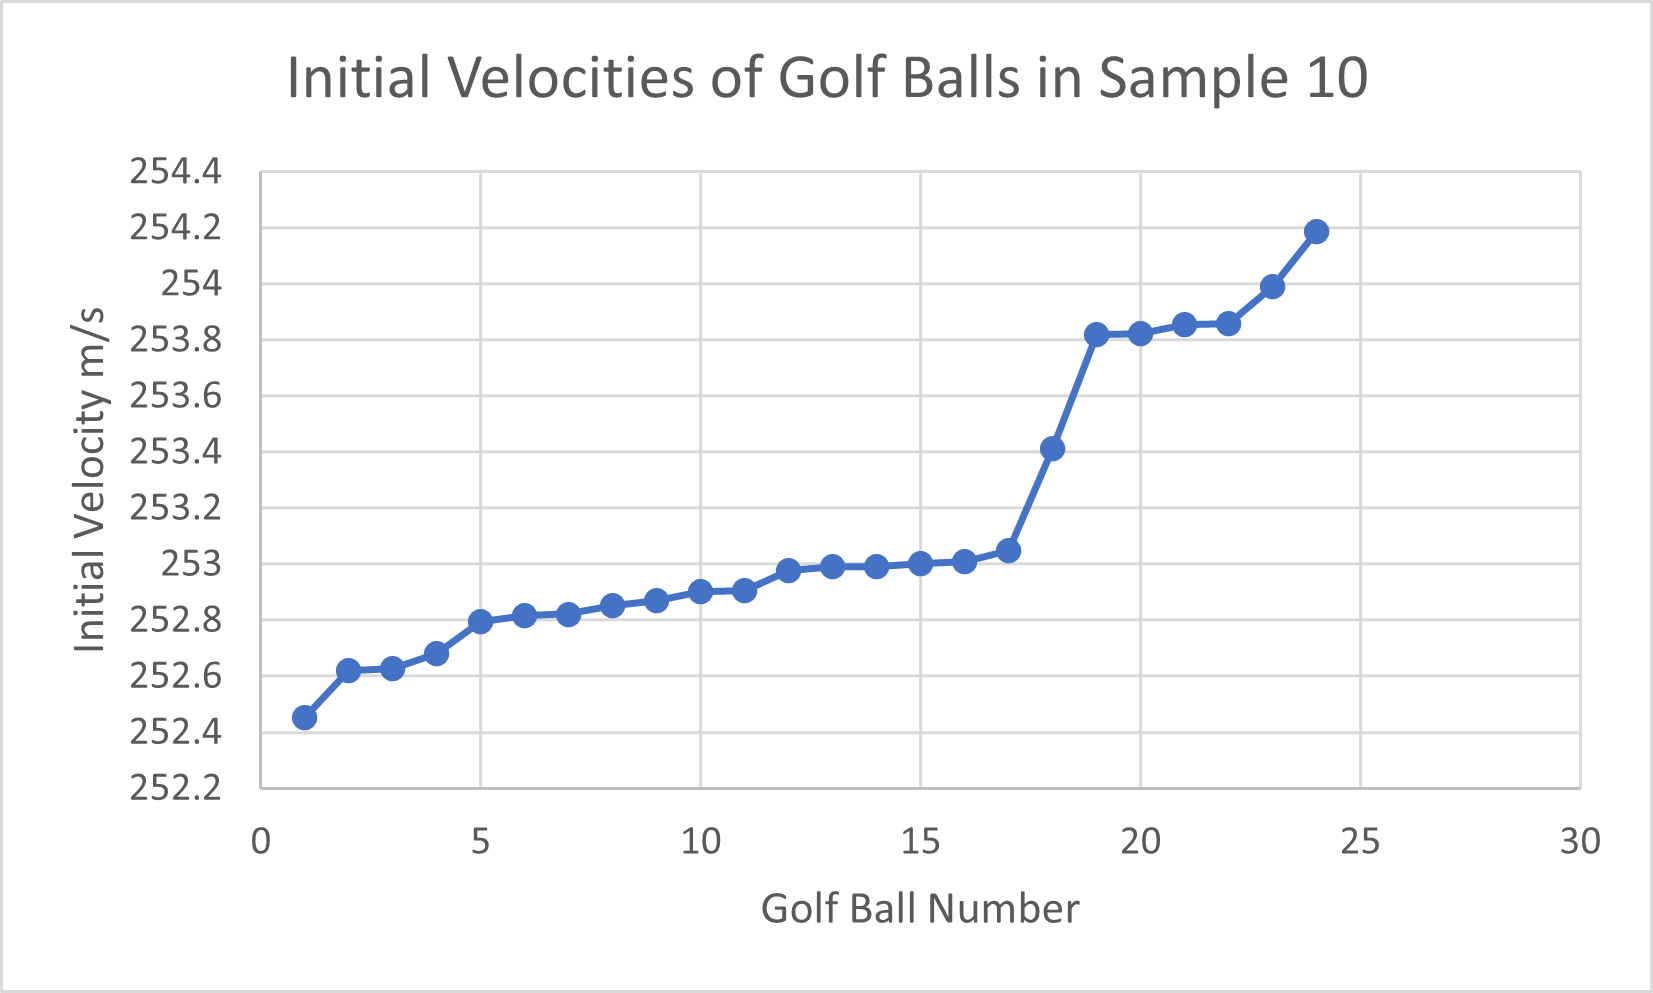
\includegraphics[width=80mm]{Sample10.png}
    \caption{Graph showing the bimodal nature of sample 10}
    \label{figure 8}
\end{figure}


In cases such as these, it would be better to model the velocities with 2 normal distributions rather than 1. Now supposing a competitor were allowed to use golf balls from such a sample, then they may be able to identify which balls in the sample perform according to which distribution and exploit this distinction to work around the 'One Ball' rule.

A method is needed whereby, given a sample, we have a test to determine if it is bimodal or unimodal. If there is not enough overlap between these 2 distributions, then the test will detect that the distribution is bimodal, and indeed if there is little overlap between the distributions, then the golf balls from the sample cannot be considered the same.

Holzmann and Vollmer\cite{Analysis} outline a criterion for unimodality. If a sample is suspected of being bimodal, following 2 means $\mu_1$ and $\mu_2$, and 2 standard deviations $\sigma_1$ and $\sigma_2$, then the sample is unimodal if and only if:

$$\frac{|\mu_1-\mu_2|}{2\sqrt{\sigma_1\sigma_2}}\leq1$$

By inspecting this inequality, we understand it as a measure of the overlap of the 2 candidate distributions. The smaller the distance between the means becomes, the more overlap we will see, and the smaller the numerator will become, bringing us closer to satisfying the condition for unimodality. Also, the larger the standard deviations are, the more spread out the distributions are and so the greater the overlap will be. Indeed this would make the denominator larger, once again bringing us closer to satisfying the condition. 

But to do this, candidate means and standard deviations of the 2 normal distributions need to be known, rather than the mean and standard deviation of the whole sample. So it needs to be determined which data points should be counted in which distribution. 

For it to be sensible to consider a bimodal distribution, we would expect a 'large' jump between consecutive values. Indeed if there were no large jumps, then a unimodal model would be perfectly sensible. By computing the differences in velocity between successive data points, we can form a distribution of the size of the gaps in the initial velocity from one golf ball to the next. In the case of sample 10 above, the largest jump is from ball 18 to 19, so we will split the 2 distributions here. That is, we will take $\mu_1$ and $\sigma_1$ as the mean and standard deviation of the balls 1 to 18, and $\mu_2$ and $\sigma_2$ for balls 19 to 24.


After doing this, we compute:

$$\mu_1=252.8757\;\;\;\;\;\;\;\;\sigma_1=0.20349$$
$$\mu_2=253.9226\;\;\;\;\;\;\;\;\sigma_2=0.131527$$


\begin{figure}[H]
    \centering
    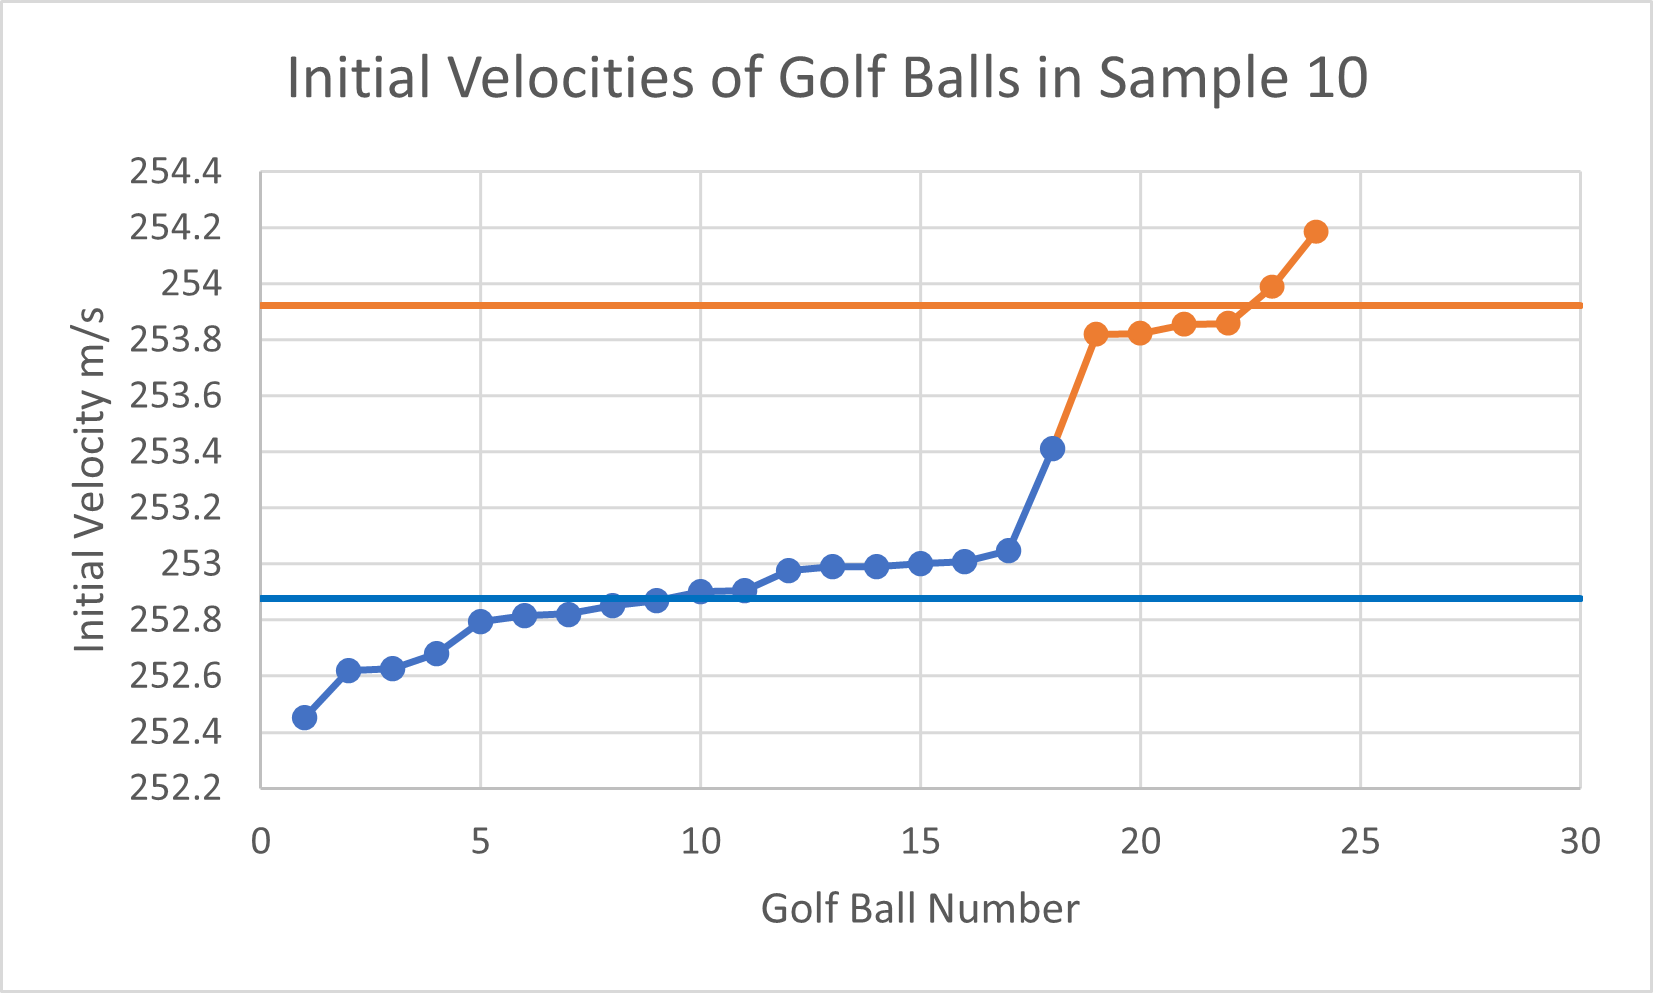
\includegraphics[width=80mm]{Sample10bimodal.png}
    \caption{Graph showing the subgroups of sample 10, and the respective means of the subgroups}
    \label{figure 9}
\end{figure}


Substituting these values in yields

$$\frac{|\mu_1-\mu_2|}{2\sqrt{\sigma_1\sigma_2}}=3.19960>1$$

So according to the above condition, sample 10 ought not be considered as a single unimodal distribution, rather a bimodal distribution- the amalgamation of two normal distributions. Since there is little overlap between the distributions, having failed the test for unimodality, we can conclude that golf balls from Sample 10 cannot in general be considered the 'same' as there is too much inconsistency within the sample. The same criterion can be applied to other samples displaying a similar bimodal or multimodal property to determine quantitatively if the differences are indeed significant enough to deem a sample of golf balls the same or different.





\section{Comparing Year to Year}
%we assume samples 51-100 are the second year samples. comparing the mean of the two samples and how each value changes for lowest, 2nd lowest, .... and take an average of difference. if this average is small enough, then there is sameness
Since it wasn't specified what year the samples were from, we are going to make the assumption that the samples labelled $1$ to $50$ are from Year 1, and the sample labelled $51$ to $100$ are from Year 2.

We can compare the two year data sets in numerous ways and analyse many important values (e.g. mean, median, interquartile range). One way at comparing data is looking at it graphically. First, we calculate the mean averages of the golf balls velocity from each sample. Then, we order these values from smallest value to largest. We can graph the two sets of data on a comparative scatter graph, and plot the two sets of data against each other to see how similar the shape of the scatter graphs are.


\begin{figure}[H]
    \centering
    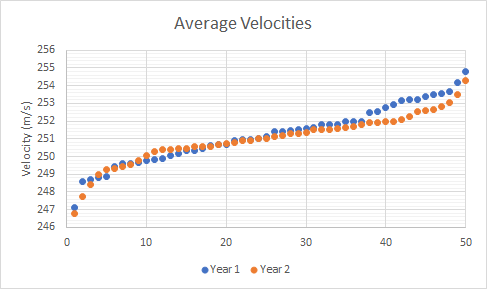
\includegraphics[width=80mm]{Average Velocities.png}
    \caption{Average Velocities of Year 1 and 2}
    \label{figure 10}
\end{figure}
\begin{figure}[H]
    \centering
    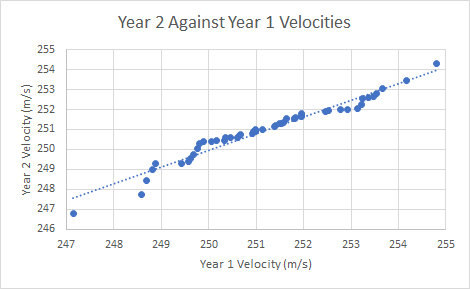
\includegraphics[width=80mm]{Scatter Graph.png}
    \caption{Year 2 plotted against Year 1}
    \label{figure 11}
\end{figure}

As we can see from these two graphs, the two years have very similar shapes. But to find out how similar the to data sets are, we could calculate the Pearson's correlation coefficient.\cite[~pg.107]{Definition}

$$r=\frac{\sum{(x_i-\bar{x})(y_i-\bar{y})}}{\sqrt{\sum(x_i-\bar{x})^2\sum(y_i-\bar{y})^2}}$$

When inputting the values into the equation, the coefficient equals 0.9767 which shows that the shape of the curves are very similar and that they are strongly correlated in the positive direction. 

However, just because they have similar shapes, doesn't mean they have the same conditions. For example, if you compare data that have values 1,2,4 and 100,200,400, they would have a Pearson's coefficient of 1 but would seem vastly different. Thus, we would have to look into the differences between $x_i$ and $y_i$ (where $i$ is between 1 and 50) and average them. If it is a small enough value, we can be fairly confident to say that they are from the same company.

\begin{figure}[H]
    \centering
    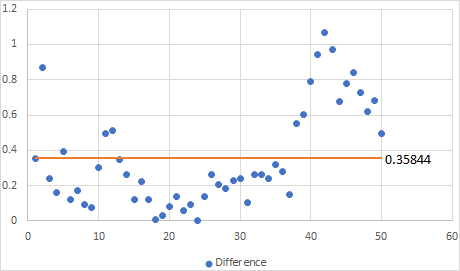
\includegraphics[width=80mm]{Difference.png}
    \caption{Differences of Year 1 and Year 2}
    \label{figure 12}
\end{figure}

As we can see from the graph, the average value for the difference between Year 1 and 2 is $0.358$. This means, on average, the $i^{th}$ value of Year 2 is $\pm0.358$ from Year 1. We can also divide this by the range of Year 1 and 2 to see how much this change is as a percentage. This turns out to be $2.9\%$ which is fairly small and would suggest that there is sameness.

We can also compare the distribution of the two sets to see how the velocity of the balls have changed. We can do this by plotting histograms of the the data sets with identical class intervals. In this case, there are 9 intervals of constant width from 246 to 255.

\begin{figure}[H]
    \centering
    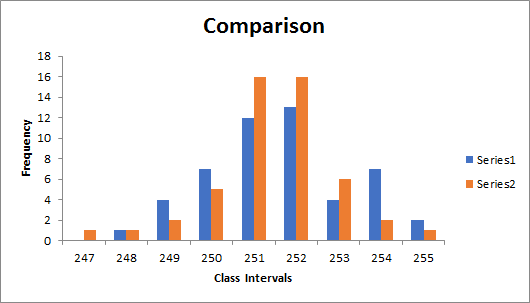
\includegraphics[width=80mm]{Comparison Histogram.png}
    \caption{Distribution of Year 1 and Year 2}
    \label{figure 13}
\end{figure}

From the two graphs, what is shown is that Year 1 and Year 2 have almost normal distribution with only slight skews. However, we can tell that Year 2 has more concise data. This can also be shown from a box plot.

\begin{figure}[H]
    \centering
    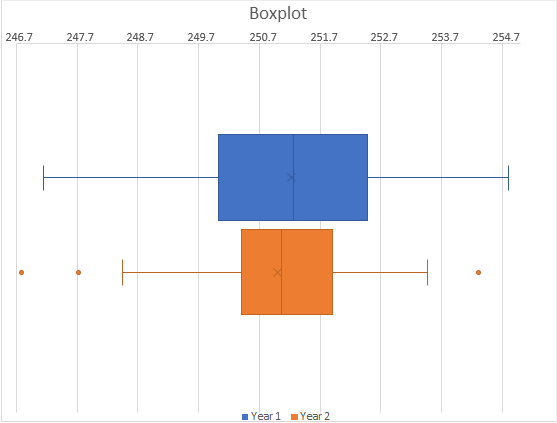
\includegraphics[width=80mm]{Boxplot.png}
    \caption{Boxplot of Year 1 and Year 2}
    \label{figure 14}
\end{figure}

The interquartile range of Year 2 is smaller(i.e. more concise data). We can deduce the skew of the two years as well. Year 1 and Year 2 is skewed to the right, meaning they both have positive skew. However, the mean is less than the median. This is due to extreme values towards the left side affect the mean to be lower than the median since outliers effects on the mean the most out of all the averages.

\section{Conclusion}
It is clear that, in professional play, the conformity of the golf balls is vital in order to preserve the integrity of the game and, further, the tournament. Of course, it is then also incredibly important for respected organisations such as the R\&A to place the same amount of importance on their golf ball conformance tests. If the performance of a certain model of golf ball is inconsistent, the ball may perform differently, and give the golfer an advantage, under different conditions such as the weather, or humidity.

In this report, many different indications that a golf ball may be performing inconsistently, have been identified. These include a large range of initial velocities, a large number of data points deemed to be 'outliers', subgroups within a sample, or the 'same' model of ball performing differently from year to year. Of course, the R\&A must set strict guidelines for these balls to be deemed suitable, and once a mathematical test has been developed, it should be adapted in order to make the test more accurate and efficient. By developing these methods, we have been able to outline a criteria against which each model of golf ball can be judged, in such a way that is easily comprehended, easily computed and, above all, accurate to a high degree. 

\newpage

\printbibliography

\end{document}
